
\section{SECDA-LLM}

SECDA-LLM is a specialized platform for creating FPGA-based LLM accelerators for edge devices using the SECDA methodology~\cite{harisSECDAEfficientHardware2021} within the \LPP environment.
Figure~\ref{fig:secda_llm} outlines the main components of SECDA-LLM.
The platform simplifies the accelerator design process by integrating the SECDA tools (e.g., AXI-API, profiler) , thus allowing a seamless connection between the SECDA design environment and the target application framework, \LPP.
This integration enables developers to begin prototyping and integrating their new accelerator designs with minimal setup costs.


\begin{figure}[!ht]
 \centering
 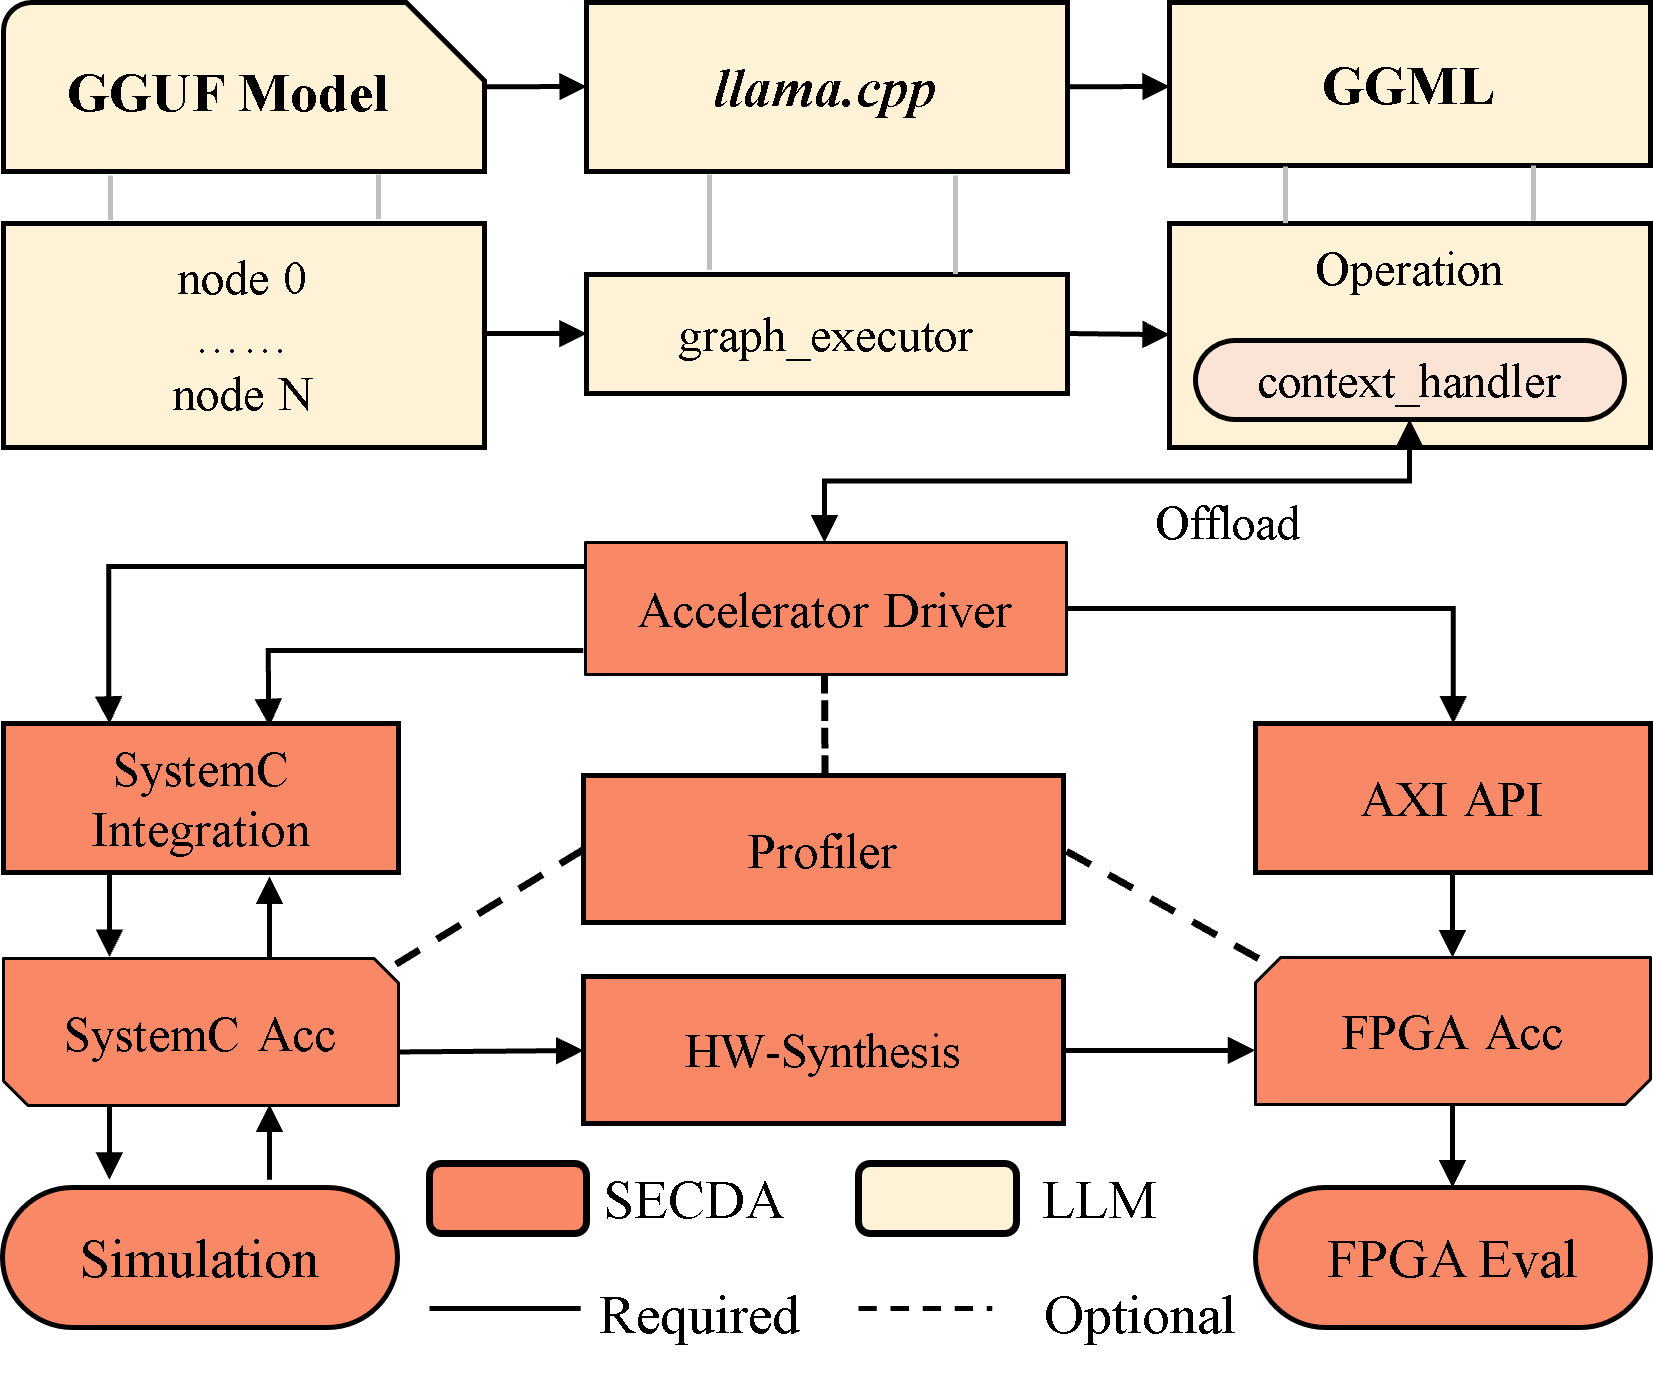
\includegraphics[width=0.9\columnwidth]{files/secda_llmv2.png}
  \caption{\label{fig:secda_llm} Overview of SECDA-LLM. Key SECDA components are highlighted in orange, and the LLM components are highlighted in beige.}
\end{figure}


% The rest of this section provides details on SECDA-LLM and: i) how it is integrated with \LPP; ii) how it enables the accelerator designer to prototype and simulate new designs with SystemC~\cite{IEEE2012systemc} simulation; iii) the ease of hardware evaluation; iv) the profiling and performance analysis capabilities of SECDA-LLM.

The rest of this section provides details about SECDA-LLM at:
\begin{enumerate*}[label=\roman*)]
    \item how it is integrated with \LPP;
    \item how it enables the accelerator designer to prototype and simulate new designs using SystemC~\cite{IEEE2012systemc};
    \item the ease of hardware evaluation;
    \item the profiling and performance analysis capabilities.
\end{enumerate*}


%*********************************************************************************************

\subsection{Integration with \LPP}

Figure~\ref{fig:secda_llm} shows that SECDA-LLM builds upon the core \LPP project.
Our current integration is through \LPP's `main' example project, which enables users to run LLMs with minimal overhead.
We can connect into \LPP once it calls any of the \GGML's operations.

Depending on our target operation(s), we create additional connection points from the \GGML library to the SECDA environment.
During these connections, we ensure the creation of a context handler to pass from the \GGML environment to the SECDA environment; the context handler includes memory pointers, memory-mapped model data, access to relevant inputs tensors, quantization, and layer parameters.


%*********************************************************************************************

\subsection{SECDA Environment}

Within the SECDA components shown in Figure~\ref{fig:secda_llm}, the accelerator designer can start quickly prototyping the initial accelerator design and driver code.
First, the user is required to create the initial driver, a simple C++ class that will gain access to the context handler provided by the offload call from~\GGML.
Second, the developer must create an initial SystemC description of their accelerator.
Then, the user can instantiate their desired data communication channels between the driver and accelerator using data interfaces provided within the SECDA environment (e.g, AXI4-S, AXI-MM and AXI-Lite).
The developer can use these data channels for SystemC end-to-end simulation.


%*********************************************************************************************

\subsection{SystemC Simulation}

SystemC end-to-end simulation is a crucial step in the SECDA methodology; therefore, SECDA-LLM provides access to SystemC simulation.
The simulation-based design loop is shown at the bottom left half of Figure~\ref{fig:secda_llm}.
Once the driver and accelerator are connected through the desired data communication channels, the user can perform end-to-end simulations of LLMs using SECDA-LLM.
With simulation enabled, the designer can quickly prototype new driver and accelerator features, verifying correctness, profiling performance and modeling control flow behavior within their design.
Therefore, the hardware developer is able to rapidly iterate through their design process, through end-to-end simulation, to meet the target performance.


%*********************************************************************************************

\subsection{Hardware Evaluation}

With simulation-based evaluation, the designer can quickly make fast, broad design changes.
Once satisfied with a given design, the designer can quickly take the SystemC-defined design and perform High-level synthesis (HLS) and logic synthesis (HLX) through the hardware synthesis tool provided by SECDA-LLM to map it to the target FPGA, as shown on at bottom right of Figure~\ref{fig:secda_llm}.
Additionally, as SECDA-LLM is integrated with the \LPP project, we can leverage the \LPP project's compilation flow to generate pre-defined applications that use the LLMs through the \LPP's interface.
These generated applications will now have complete access to the driver and accelerator for execution on an FPGA-enabled device; see Section~\ref{subsubsec:exp_setup} for details.

A major benefit of the SECDA methodology, and therefore SECDA-LLM, is that we can reuse the driver and accelerator completely.
Therefore, for actual FPGA evaluation the designer does not need to make any changes to the driver to enable real hardware execution, as the SECDA data interfaces switch between simulation and FPGA execution through a simple \textit{"SYSC" }compiler flag.
Once the accelerator is mapped to the target FPGA, the designer can evaluate its performance with their target applications.


%*********************************************************************************************

\subsection{Profiling}

% Through SECDA-LLM, we provide two types of profiling: simulation profiling and execution time profiling, these two types of profiling are enabled by the "Profiler" module shown in figure~\ref{fig:secda_llm}.

Through SECDA-LLM, we provide two types of profiling: simulation profiling and execution time profiling.
The \emph{profiler} module shown in Figure~\ref{fig:secda_llm} highlights how the profiling interacts with both the accelerator design and driver.
Additionally, we are able to leverage any additional profiling tools provided by the \LPP project.


\subsubsection{Simulation profiling}

End-to-end SystemC simulation can be used to quickly evaluate the potential performance impact of changes to the hardware and software components of the accelerator design and verify the correctness of the implementation.
To profile the end-to-end simulation, the developer typically needs to add additional profiling code to keep track of hardware and software metrics throughout the end-to-end LLM inference.
The \emph{profiler} module provided within SECDA-LLM enables the quick and easy method to set up capture points to profile from the accelerator.
The capture points can record different metrics of the accelerator and hardware submodules.
Metrics include clock cycle counts and the dynamic utilization of processing elements and accelerator buffers.


\subsubsection{Execution profiling}

During the hardware evaluation, SECDA profiling provides execution time for the custom driver and accelerator.
This type of profiling helps the designer understand the performance bottlenecks caused by driver-accelerator interactions.
For instance, a designer may opt to profile time spent:
\begin{enumerate*}[label=\roman*)]
    \item Sending input data;
    \item Waiting for the accelerator to execute operations;
    \item Unpacking output data received from the accelerator.
\end{enumerate*}
The analysis of these detailed execution time breakdowns can motivate both accelerator and driver design choices.
Additionally, execution profiling of an FPGA evaluation run can be used to profile driver execution times, which can be combined with SystemC-reported simulation times for the accelerator.
This would estimate end-to-end execution time in terms of both CPU and accelerator.




% During the hardware evaluation, SECDA profiling can be enabled to provide an execution times for the custom driver and accelerator.
% This could help the designer understand the bottlenecks in performance different components of driver-accelerator interactions.
% For example, the designer can choose to profile the time spent sending input data, time spent wait for accelerator to execute operations and also time spent unpacking output data received from the accelerator.
% Analysis of these detailed execution time breakdowns can motivate design choices for both accelerator and driver.
% Additionally wall clock profiling can be used during simulation run to profile driver execution times, which can be combined with SystemC reported simulation times for accelerator.
% This would provide an estimate of end-to-end execution time in terms of both CPU and accelerator.






% \subsection{Runtime Model}
% Once inside the SECDA environment, the accelerator driver obtains access to the context handler in order appropriately offload compute operation of the target node to the accelerator.
% The accelerator driver, first checks if our accelerator
% \subsection{Float based-Quantization support}


